\section{Story}

\begin{center}
  \begin{figure}[H]
    \centering
    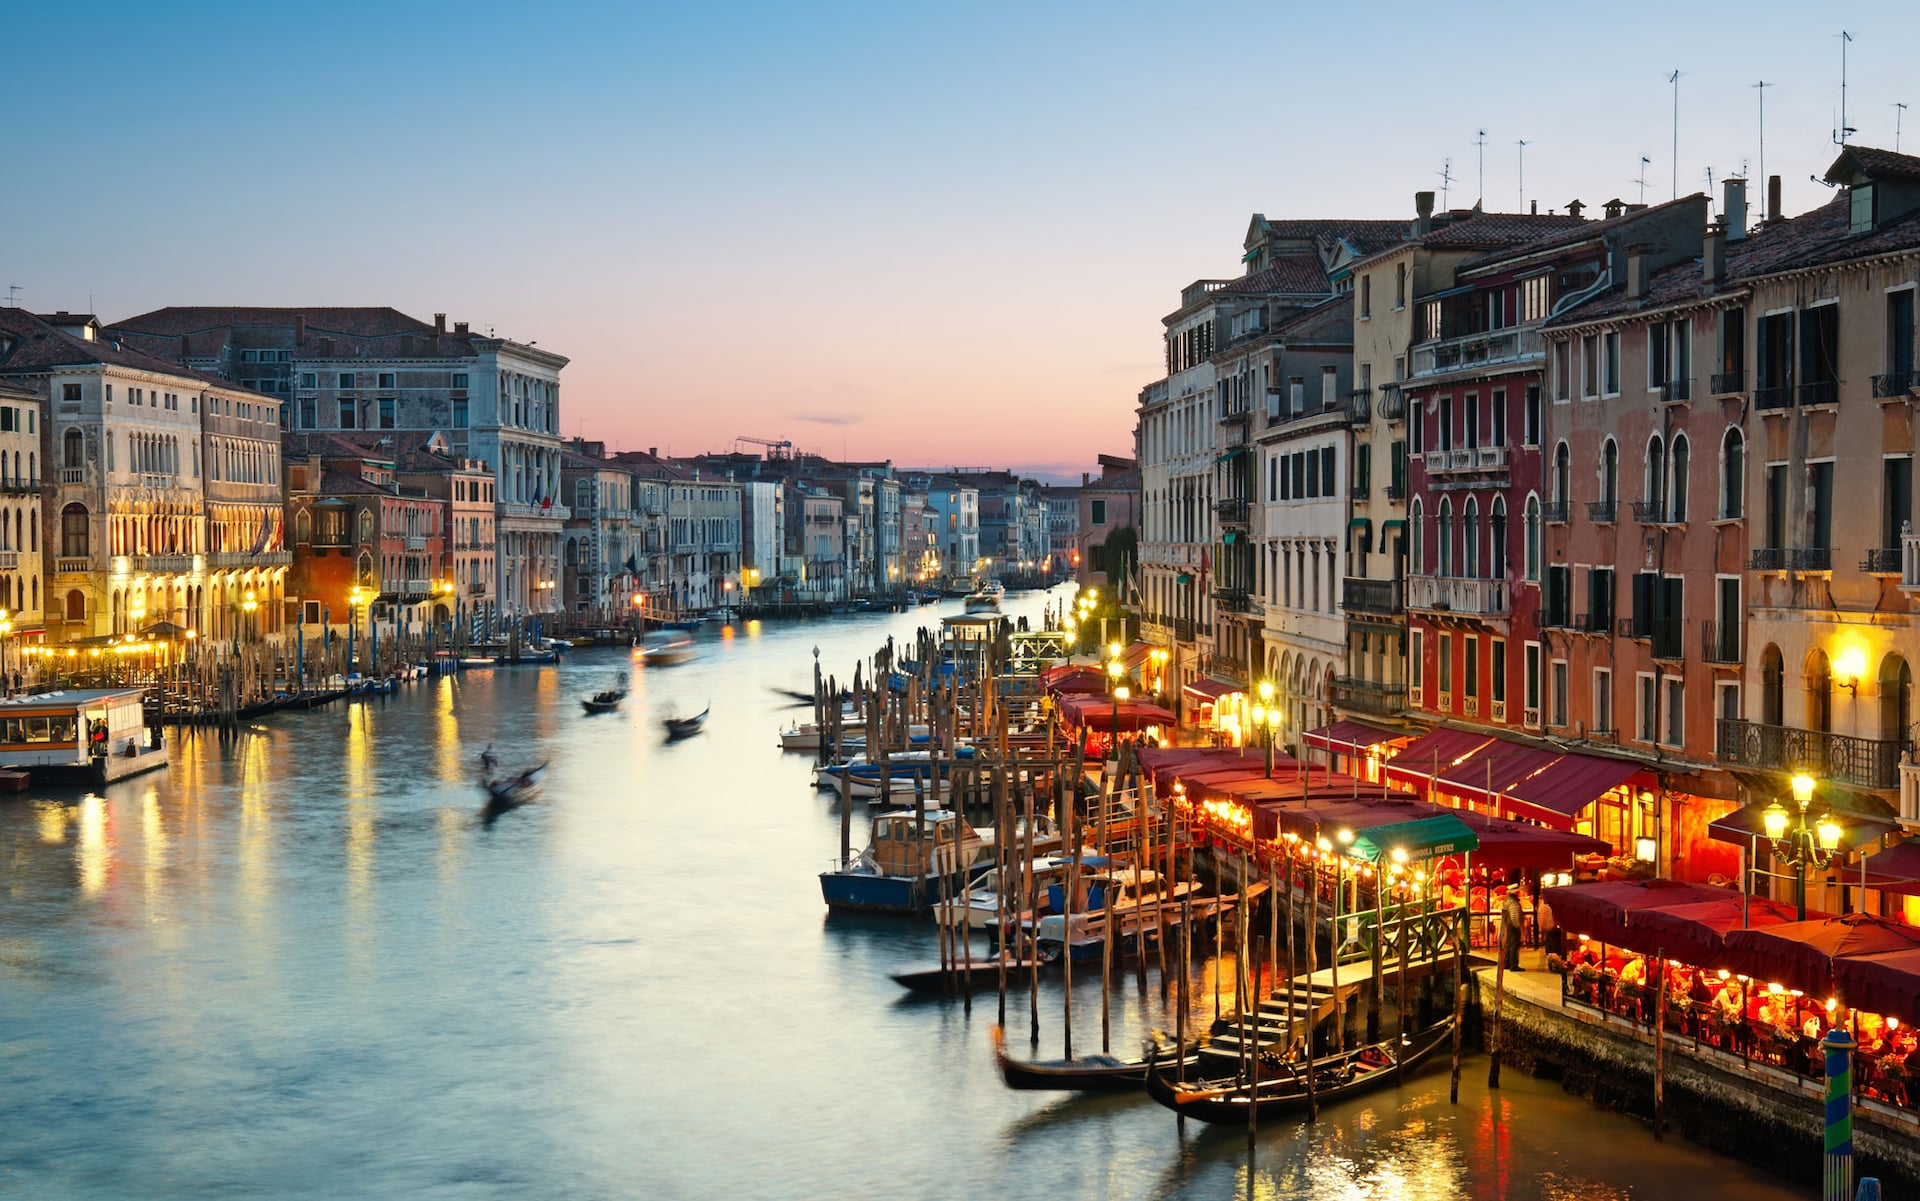
\includegraphics[width=\textwidth]{../../References/Images/Dynamia/venice-restaurants-by-canal}
    \caption{Reference image for Dynamia}
  \end{figure}
\end{center}

When Sophie and Calcifer arrive in Dynamia it is late afternoon. They find themselves in a dead end in the suburbs of Dynamia.\\

\textbf{Calcifer}: What’s this smell!?\\

\noindent They exit from the dead end moving on to a street crossed by a canal. They can hear the noise of the water on their way.

\begin{screenplay}
\extslug[afternoon]{Dynamia}

The camera  moves around Sophie to show streets and canals. 

\begin{dialogue}[amazed]{Sophie}
This city is so beautiful!
\end{dialogue}

The camera rises up to show the city, suggesting them the possible paths and, eventually,  zooming on the location of the castle. The camera rotates and returns behind Sophie's shoulders. 

\begin{dialogue}[worried]{Calcifer}
Look how much water! Be careful! Don’t let me fall!
\end{dialogue}
\end{screenplay}

\noindent \\

\textbf{Sophie (discouraged)}: Dynamia is so big! Where Howl could be?

\textbf{Calcifer}: I can’t feel his magic. He could be anywhere.

\textbf{Sophie (resolute)}: We need information. We can try to find some at the market. \\

\noindent [An indicator appears in the map.]\\

\textbf{Calcifer}: Okay. Do you think that they sell also a little bit of wood?\\

\noindent On the way, Sophie sees a manifest representing a dark-skinned woman with a crown. She can talk to it.\\

\textbf{Sophie}: Hello, maniffst. Who is this woman?

\textbf{Manifest (solemn)}: She is our enlightened and beloved Queen regent. Long live the Queen!\\

\noindent Sophie and Calcifer go to the market. There are two guards on their way.

\textbf{Sophie}: Some guards! Better not be seen.\\

\noindent They move past the guards and they reach the market, which is located in a huge crowded square where they can hear the buzz of the crowd and the shouting of the merchants in the background

%%%%%%%%%%%%%%%%%%%%%%%%%%%%%%%%%%%%%%%%%%%%%%%%%%%%%%%%

\noindent Sophie arrives at the stand in the market pointed by the indicator and finds a merchant that sells fabrics and accessories.
Sophie buys a bit of wool to make new hats.\\

\textbf{Sophie (thinking)}: This will be perfect for my hats!

\textbf{Sophie}: How affairs are going on? Do you have problems due to war?

\textbf{Merchant (resigned)}: Sure, like any other merchant. What about you? What a lonely girl is doing here?\\

\noindent \textit{Choice: two way}:
\begin{enumerate}
\item \textit{Lie}:\\
  
  \textbf{Sophie}: I work out of city, it is very hard there too. I hope the war will end soon.
  
  \textbf{Merchant (low level voice)}: Be careful, the guards could hear you.
  
  \textbf{(normal level voice)}: The prince Justine was imprisoned for this cause.
  
  \textbf{Sophie (worried)}: Imprisoned? Where? 

  \textbf{Merchant}: Obviously in the castle. Why are you so worried? Are you in league with the prince? Guards!!!!

  Two guards comes to the market but Sophie runs away before them are arrived and so sows them easily.
  
\item \textit{Bribe him}:\\
  
  \textbf{Sophie (Persuasive)}: I’m a foreigner, may you give me some information about Dynamia in war? I can pay you.
  
  \textbf{Merchant}: How much?
  
  \begin{enumerate}
  \item Sophie gives 50 coins to the merchant.\\

    \textbf{Merchant(annoyed)}: It’s not enough. Don’t waste my time!\\

    \noindent Sophie goes away disconsolate.

  \item Sophie gives 100 coins to the merchant.\\
    
    \textbf{Merchant}: Okay. I’ll tell you all I know. After the prince Justin was imprisoned ...

    \textbf{Sophie (incredulous)}: Wait, wait, wait! What? Justine was imprisoned?!
    
    \textbf{Merchant}: Yes, he tried to persuade the queen to end the war and was accused of high treason.
    
    \textbf{Sophie}: really? And where is he now?
    
    \textbf{Merchant}: Obviously, in the prison of the castle.
    
    \textbf{Sophie(hasty)}: okay, okay thank you! I have to go!!

    \noindent Sophie heads to the castle.
  \end{enumerate}
\end{enumerate}
%%%%%%%%%%%%%%%%%%%%%%%%%%%%%%%%%%%%%%%%%%%%%%%%%%%%%%%%%%%%%%%%%%%%%%%%%%%%%
\noindent Sophie and Calcifer walk down the main street, but they suddenly see a demon who is looking around.

\begin{screenplay}
\extslug[afternoon]{Dynamia}

Sophie and Calcifer hide behind a corner. 

\begin{dialogue}[worried]{Sophie}
Oh no, that’s a demon!
\end{dialogue}
\begin{dialogue}[feisty]{Calcifer}
Don’t worry, leave it to me!
\end{dialogue}

Sophie looks up at a side street.

\begin{dialogue}{Sophie}
I think we should avoid it.
\end{dialogue}

\begin{dialogue}{Calcifer}
...Or fight it!
\end{dialogue}
\end{screenplay}

%%%%%%%%%%%%%%%%%%%%%%%%%%%%%%%%%%%%%%%%%%%%%%%%%%%%%%%
\textit{Choice: two way}
\begin{enumerate}
  \item Sophie and Calcifer choose to fight the demon.
  \item Sophie and Calcifer go through another way.
\end{enumerate}
  
\noindent Sophie and Calcifer reach the main square. On one side there is the castle, on the other side the is the lagoon.
In the square there are many people and some newsboys.\\

\textbf{Newsboy}: Breaking news! Prince of Strangia accused of high treason and sentenced to death. Tomorrow morning the public execution!

\textbf{Sophie}: Oh no, we must hurry.

The castle is surrounded by the walls and the gate is patrolled by many guards.\\
%%%%%%%%%%%%%%%%%%%%%%%%%%%%%%%%%%%%%%%%%%%%%%%%%%%%%%%

\textbf{Sophie}: We cannot pass by this way, they’ll spoil us. Better find another way.\\

\noindent If Sophie tries to go through the gate, the guards will block her.\\

\textbf{Guards}: Hey, where are you going?\\

%%%%%%%%%%%%%%%%%%%%%%%%%%%%%%%%%%%%%%%%%%%%%%%%%%%%%%%

\noindent Sophie and Calcifer walk along the walls until they find a point where there are some sloping bricks.
Nearby there is a pile of old debris.\\

\textbf{Calcifer}: Hey, I can use them!

\textbf{Sophie}: Use for what?

\textbf{Calcifer (proud)}: Just wait and see.\\

\noindent Sophie comes closer to the pile and Calcifer draws him the debris to create a four-legs platform.
Sophie jumps on the mechanism and Calcifer climbs the wall thanks to the sloping bricks, then he goes down on the other side without being spotted.\\

\textbf{Sophie}: Calcifer, you are amazing!

\textbf{Calcifer (proud)}: Of course I am!

\textbf{Sophie}: Now go back to normal, they will find us in a moment.

\textbf{Calcifer (resigned)}: Yeah…\\
%%%%%%%%%%%%%%%%%%%%%%%%%%%%%%%%%%%%%%%%%%%%%%%%%%%%%%%

\noindent Sophie and Calcifer cross the courtyard of the castle careful not to be spotted by the guards (now hostile) and the demons.
They reach a wood door. It is close, but Calcifer eats it and they can proceed. They find themselves in a dark and dusty storage. They don’t see anyone inside.\\

\begin{screenplay}
\extslug[afternoon]{Dynamia: Old chicken of the castle}

Sophie and Calcifer hide behind a corner. 

\begin{dialogue}{Sophie}
Hello…?
\end{dialogue}
\begin{dialogue}[cheerful]{Objects}
 Hello!
\end{dialogue}
\begin{dialogue}{Box 1}
 Finally someone has come!
\end{dialogue}
\begin{dialogue}{Can 1}
 Do you want some beans?
\end{dialogue}
\begin{dialogue}{Can 2}
Or some tuna?
\end{dialogue}
\begin{dialogue}[worried]{Sophie}
Ssh! Shut up!
\end{dialogue}
\begin{dialogue}{Sophie}
Thank you, I’m fine. Can you tell me where is the prison?
\end{dialogue}
\begin{dialogue}{Can 2}
Over the door! (the pot indicates it)
\end{dialogue}
\begin{dialogue}{Box 2}
There are stairs that bring directly to the prison!
\end{dialogue}
\begin{dialogue}{Can 1}
But there are a lot of guards!
\end{dialogue}
\begin{dialogue}{Box 1}
Be careful!
\end{dialogue}
\begin{dialogue}{Sophie}
Do you know something about a powerful magician called Howl?
\end{dialogue}
\begin{dialogue}{Can 2}
Howl?
\end{dialogue}
\begin{dialogue}{Box 1}
Sorry, we don’t know any Howl.
\end{dialogue}
\begin{dialogue}{Can 1}
But we heard about a wizard!
\end{dialogue}
\begin{dialogue}{Sack 1}
Yesterday we heard two guards talking about a powerful wizard.
\end{dialogue}
\begin{dialogue}{Box 2}
He has been defeated by the queen regent and he has been imprisoned in spirits realm.
\end{dialogue}
\begin{dialogue}{Calcifer}
Oh no, I knew he was in danger.
\end{dialogue}
\begin{dialogue}{Sophie}
My poor Howl! I’m so frightened for him. Wait, where do you say he is?
\end{dialogue}
\begin{dialogue}{Box 2}
The spirits realm.
\end{dialogue}
\begin{dialogue}{Box 1}
Or something like that.
\end{dialogue}
\begin{dialogue}{Can 1}
We don’t know.
\end{dialogue}
\begin{dialogue}{Can 2}
We are just cans!
\end{dialogue}
\begin{dialogue}{Sophie}
Ok, ok. Thank you very much. Now we have to go.
\end{dialogue}
\begin{dialogue}{Sack 1}
Watch out for the queen regent.
\end{dialogue}
\begin{dialogue}{Box 1}
She is very powerful.
\end{dialogue}
\begin{dialogue}{Can 1}
And dangerous!
\end{dialogue}
\begin{dialogue}{Can 2}
Stay away from her!
\end{dialogue}
\end{screenplay}

\noindent Sophie and Calcifer follow the indication of the object and they reach the prison. In front of the passage there are two guards talking.\\

\textbf{Guard 1}: Sorry I’m late, now you can go home.

\textbf{Guard 2}: Thank, I’ll change my clothes and leave.\\

\noindent Sophie and Calcifer stay hidden and they let the guard 2 move on, while the guard 1 keeps patrolling the passage.\\

\textbf{Sophie}: Maybe we can follow that guard and steal his clothes when he’s gone.\\

\textit{Secondary mission}: the player can follow the guard 2 until the locker room and take his clothes when he is gone, otherwise he/she can attack the guard on the way.

\textit{Reward:} guard clothes for Sophie. When Sophie wears them, it takes longer for the guards to spot her after they have seen her.\\

\noindent After the mission, the player returns to passage to the prison.\\

\textbf{Calcifer}: Leave it to me, I’ll knock him down in a moment!

\textbf{Sophie}: Wait, maybe there is another passage.\\

\textit{Choice: two way}:
\begin{enumerate}
\item Sophie attacks the guard with Calcifer.
\item Sophie goes back:\\

  Sophie goes back upstairs and she follows the corridor. She finds other stairs that bring to the prison entrance. There there is an old and rusty torch.\\
  
  \textbf{Calcifer}: Time to fight?\\

  \noindent Sophie looks the torch. Sophie (to the PortaTorcia at low voice): Pss. I need your help.\\

  \textbf{Torch (tired)}: Whaaat? Meee?

\textbf{Sophie (at low voice)}: Yes, please. Can you help me?

\textbf{Torch (tired)}: Of cooourse. What can I doooo?

\textbf{Sophie}: Just count to twenty and then fall down.

\textbf{Torch (tired)}: Fiiiiine.\\

\noindent Sophie goes back upstairs and then she goes down on the opposite site. The torch falls down and the guard, alarmed, leave his position to check out the situation.
Sophie can pass through without being spotted.
  
  \end{enumerate}

Sophie and Calcifer reach the prison. There are many occupied brigs, but they don’t find Justin.
Sophie talks with a torch.\\

\textbf{Sophie}: Excuse me, where can I find prince Justin?

\textbf{Lamp (ill-tempered)}: That worm is in the darkest and wettest brig. That way. Do you wanna join him?

\textbf{Sophie}: By any chance, have you heard of a wizard? Maybe he has been brought here.

\textbf{Lamp}: Wizard? What wizard? There’s no wizard down there. Now leave me alone. Me and my miserable job.\\

\noindent Sophie and Calcifer keep going within the prisons evading or fighting against the human and demon guards till they manage to find the Justin’s brig. They find him quite in good health and not wounded.\\

\textbf{Justin (surprised and worried)}:Sophie! Calcifer! Guys, what are you doing here !? It is so dangerous

\textbf{Sophie}: We were looking for some information about Howl, when we discovered that you had been imprisoned. You’ll be executed tomorrow!\\

\noindent They try to pick the lock of the door of the brig, then they try to melt it using Calcifer fire, but they fail repeatedly.\\

\textbf{Calcifer}: This lock is so resistant, seems enchanted!

\textbf{Justin}: Yes… I think the only way to open the door is stealing the key from tha captain of the guards, but it is too risky… Go away and stay safe, leave me alone!

\textbf{Sophie and Calcifer}: We would never let you down. Where is the captain?

\textbf{Justin}: Thanks, guys. You are true friends. The captain typically stays in the guards’ room, but I’ ve heard he keeps always the door open to look what his underlings are doing. So while he is distracted you can get in and steal the passepartout key he holds attached to his belt.\\

\noindent Sophie and Calcifer begin looking for the guards’ room, until, after few minutes, they notice an open door  at the end of a hallway\\

\textbf{Sophie and Calcifer (thinking)}: That must be the room!\\

\noindent They slowly walk towards the guards’ room, staying in the shade and hiding in blind spots to evade the guards patrolling the corridors. Once they get there, Sophie peeks inside the room and she patiently waits until the captain is turned towards the opposite direction. She slides under a big wooden table, remaining unseen. She waits again until the captain come closer to her and she grabs the key without making any noise and she quickly gets out.

Sophie and Calcifer go back to Justin and they free him.\\

\textbf{Justin}: follow me i know a secret door in the prison to go out in the courtyard. Fast! \\

\noindent While running away they hear a scream.\\

\textbf{Captain of the guards}: SOMEONE STOLE MY KEY!! FIND THE THIEF!!\\

\noindent Now the guards are on alert, so they must hurry up and run away.

Exited from the prison while they are crossing the castle courtyard the guards see them.\\

\textbf{Guard 1}: Hey what are you doing?

\textbf{Guard 2}: What? The prince is free! Notice all the guards. the prisoner is running away with a girl, let's take them!\\

\noindent Calcifer uses the debris from before to climb the walls and at this point it begins the haunting for them.
Sophie leads the way to sow the guards and Justin follow her. Running away through Dynamia, Justin notices that the guards have blocked some way and so advices Sophie.\\

\textbf{Justin}: I trust you, but i think it's difficult sow ing or fighting so many guards.
If we went to the bridge to right to the market we could crossed Dynamia with a gondola. 

\textit{Choice: two way}
\begin{enumerate}
\item Go on walking:\\
  Ingnoring the advice Sophie keeps her way until they arrive to the dead end where is placed the secret passage for the flying castle. Occasionally fighting or avoiding some guards
  \item Go to the bridge:\\
    Sophie follows the Justine advice and leads the team to the bridge.
    
Once arrived:\\

\textbf{Sophie}: Ok, Justin start the boat now. I have not driven one.

\textbf{Justin}: I’m sorry, me too.

\textbf{Sophie}: REALLY!? What we do now?

\textbf{Calcifer}: You can do it! Use your magic Sophie!

\textbf{Boat}: Hello Sophie. I’m here to help you. Tell me a cardinal point and i will move in that direction. I’m yours to command.

\textbf{Sophie}: Oh no, the guards! Start now boat! Go to North.\\

\noindent They sow the guards along the canal and dock next some suburb house. They are safe. Nearby they find the dead end where is placed the secret passage for the flying castle.
\end{enumerate}















